\documentclass[12pt]{article}
\usepackage[a4paper,margin=2.5cm]{geometry}
\usepackage{hyperref}
\usepackage{graphicx}
\usepackage{parskip}
\usepackage{enumitem}
\usepackage{longtable}
\usepackage{verbatim}

\title{Atividade 2: Auditoria Forense de Software e Plano de Resgate Tecnico}
\author{Equipe: Dean Vinícius Palmeira de Meneses; Hilton Hunaldo Costa Silva Brito \\ Projeto: langfuse/langfuse}
\date{2026-05-31}

\begin{document}
\maketitle

\section*{1. Contexto e objetivo}
Esta auditoria forense avalia a saude gerencial e arquitetural do repositorio langfuse/langfuse, com foco nos eixos do enunciado: Gestao (MPS.BR GPR), Anatomia do Codigo (SOLID/DRY) e Padroes GoF. Para cada item, apresentamos evidencia, diagnostico, classificacao de risco e recomendacao.

\section*{2. Eixo A: O Pulso da Gestao (MPS.BR GPR)}
\subsection*{A1. Arqueologia de Issues}
\textbf{Evidencia (issue e discussoes):} \href{https://github.com/langfuse/langfuse/issues/13933}{Issue \#13933} e comentarios com analise de causa e proposta de mudanca de rota (novo endpoint by-id).\\
\begin{center}
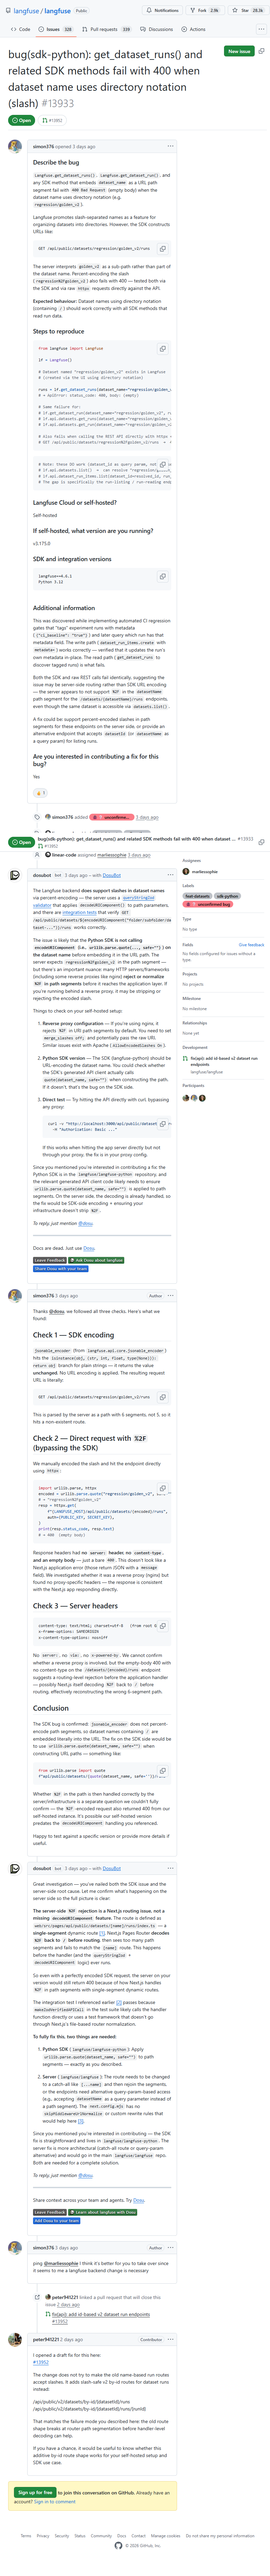
\includegraphics[width=0.92\linewidth]{prints/a1-issue-body.png}\\[0.5em]
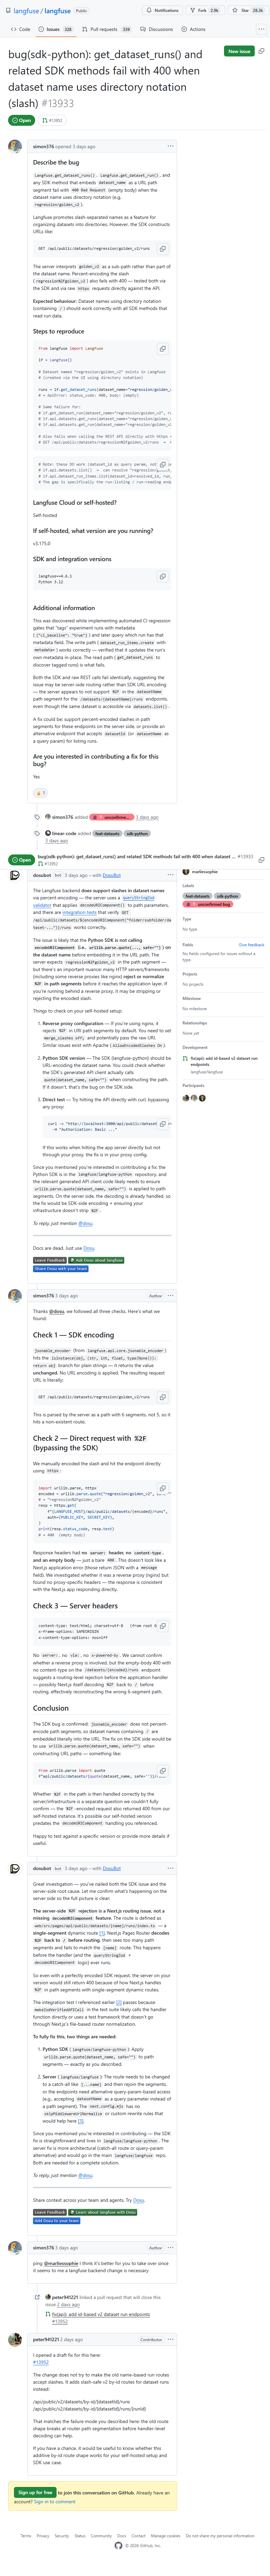
\includegraphics[width=0.92\linewidth]{prints/a1-issue-comments.png}
\end{center}

\textbf{Diagnostico:} A issue mostra investigacao tecnica detalhada, confirmando falha tanto no SDK (encoding de path) quanto na rota do servidor, e culmina em mudanca de escopo para adicionar endpoints by-id. Essa dinamica indica boa engenharia investigativa, mas revela dependencia entre repositorios (SDK + server) e impacto em compatibilidade de API.

\textbf{Risco:} Medio. A dependencia cruzada e a mudanca de escopo podem atrasar correcoes e gerar regressao se nao houver alinhamento formal.

\textbf{Recomendacao:} Formalizar criterios de aceitacao multi-repo (SDK + server), vincular issues entre repositorios e registrar a decisao arquitetural (ADR). Incluir teste de integracao cobrindo nomes com ``/'' e a nova rota by-id.

\subsection*{A2. Gestao de Riscos Ocultos (TODO/FIXME)}
\textbf{Evidencia (TODOs relevantes):}\\
\href{https://github.com/langfuse/langfuse/blob/main/worker/src/queues/otelIngestionQueue.ts#L215-L219}{otelIngestionQueue.ts L215-L219} (log de blob storage) \\
\href{https://github.com/langfuse/langfuse/blob/main/worker/src/queues/webhooks.ts#L49-L52}{webhooks.ts L49-L52} (versionamento da API de webhook) \\
\href{https://github.com/langfuse/langfuse/blob/main/worker/src/queues/webhooks.ts#L568-L570}{webhooks.ts L568-L570} (templates customizados via UI) \\
\href{https://github.com/langfuse/langfuse/blob/main/packages/shared/src/server/llm/compileChatMessages.ts#L98-L105}{compileChatMessages.ts L98-L105} (IDs de mensagens) \\
\begin{center}

\includegraphics[width=0.48\linewidth]{prints/a2-otelIngestionQueue-main.png}\hfill

\includegraphics[width=0.48\linewidth]{prints/a2-webhooks-49-52.png}\\[0.5em]

\includegraphics[width=0.48\linewidth]{prints/a2-webhooks-568-570.png}\hfill
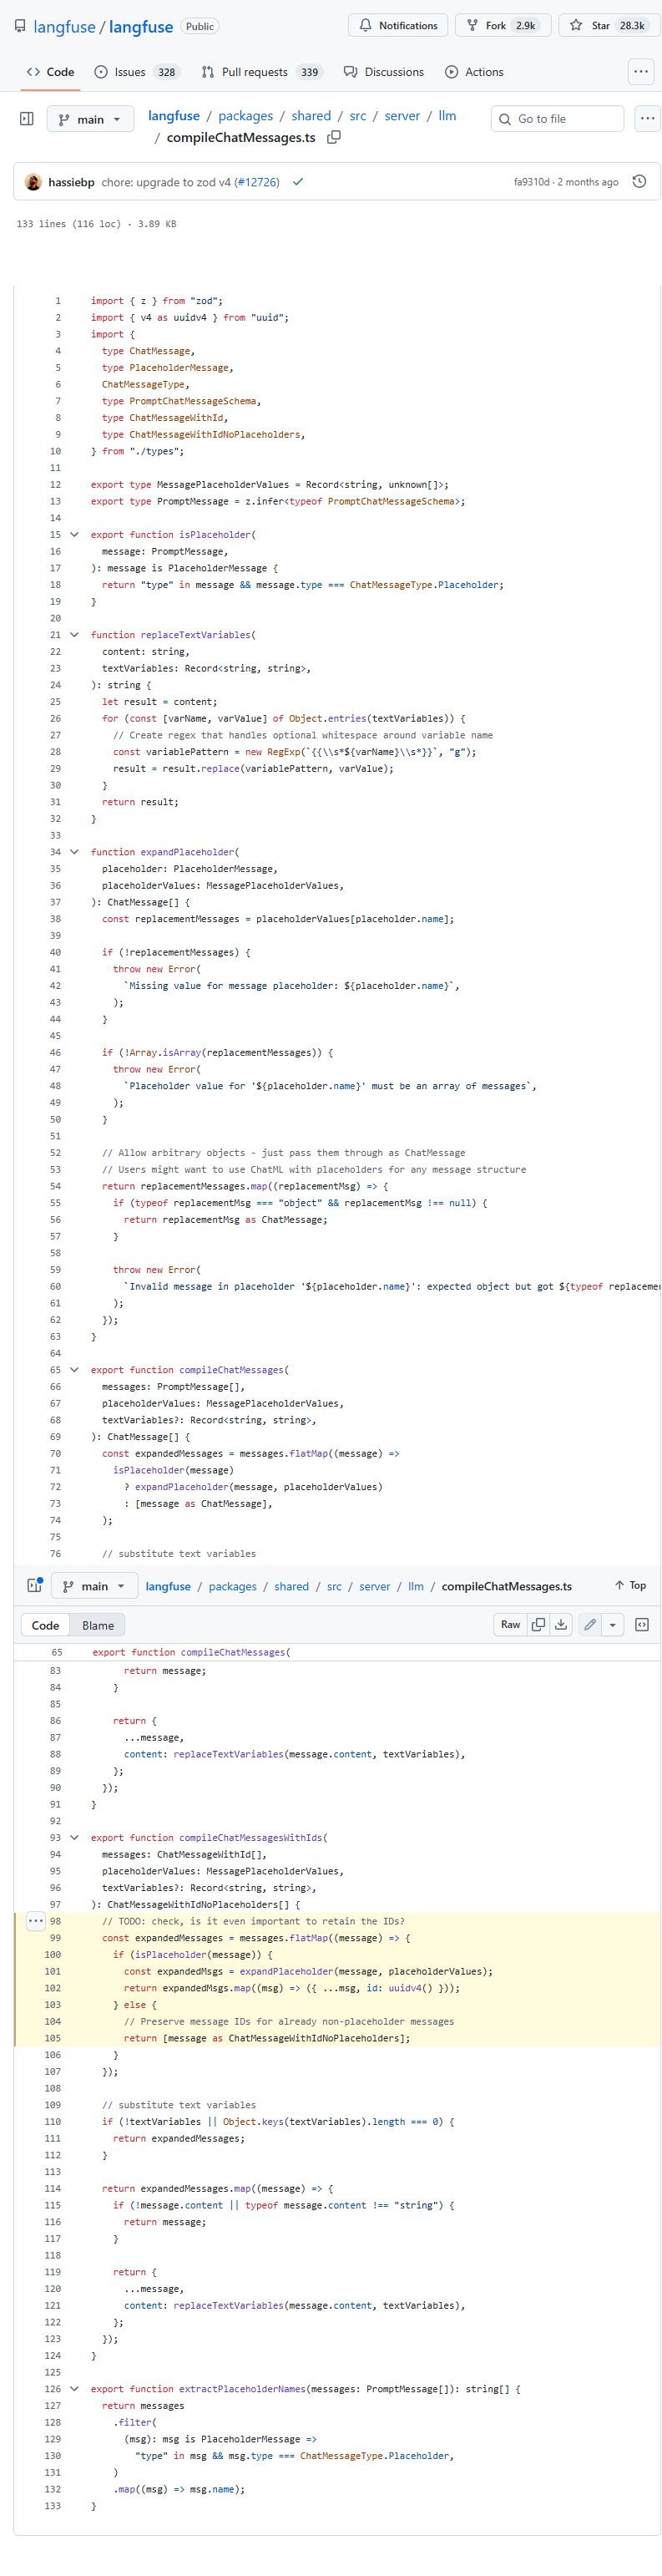
\includegraphics[width=0.48\linewidth]{prints/a2-compileChatMessages.png}
\end{center}

\textbf{Diagnostico:} Existem TODOs em filas criticas (ingestao e webhooks) e em fluxo de LLM. Sao sinais de riscos tecnicos latentes que podem impactar confiabilidade e capacidade de auditoria (ex.: log de blob storage e versionamento de webhooks).

\textbf{Risco:} Medio/Alto. Os TODOs estao em areas de integracao com terceiros e pipelines de dados.

\textbf{Recomendacao:} Criar registro de riscos com priorizacao e dono, converter TODOs em issues com data-alvo e criterios de aceite, e definir politica de ``no TODO without issue''.

\subsection*{A3. Ritmo de Entrega e Code Review}
\textbf{Evidencia (cadencia):} \href{https://github.com/langfuse/langfuse/graphs/contributors}{Grafico de contribuicoes} e \href{https://github.com/langfuse/langfuse/pulse}{Pulse}.\\
\textbf{Evidencia (code review):} comentario de follow-up indicando ajustes por feedback em \href{https://github.com/langfuse/langfuse/pull/13955\#issuecomment-4585104387}{PR \#13955}.\\
\begin{center}
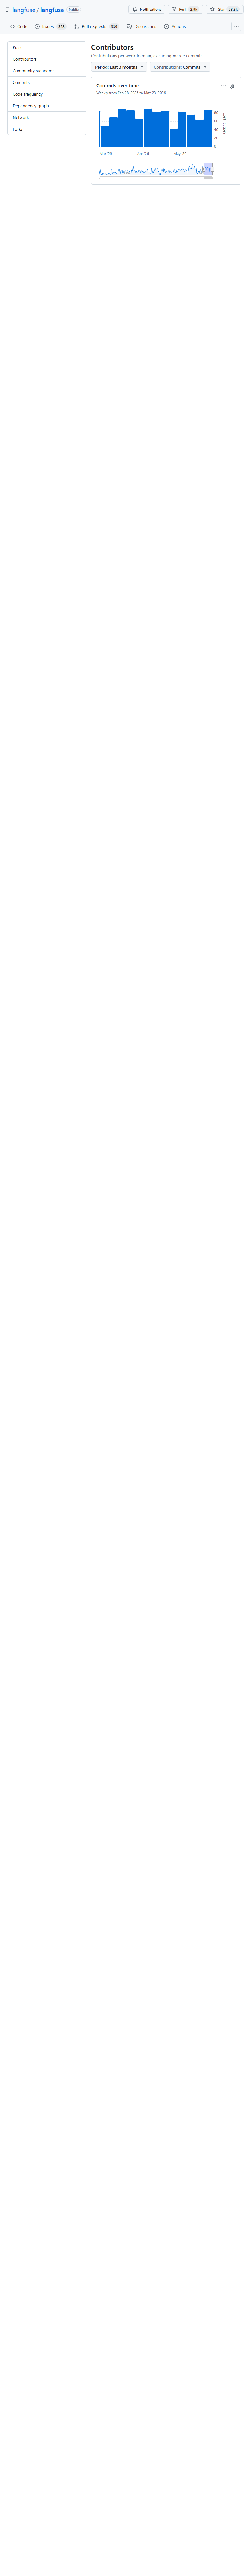
\includegraphics[width=0.48\linewidth]{prints/a3-contributors.png}\hfill

\includegraphics[width=0.48\linewidth]{prints/a3-pulse.png}\\[0.5em]
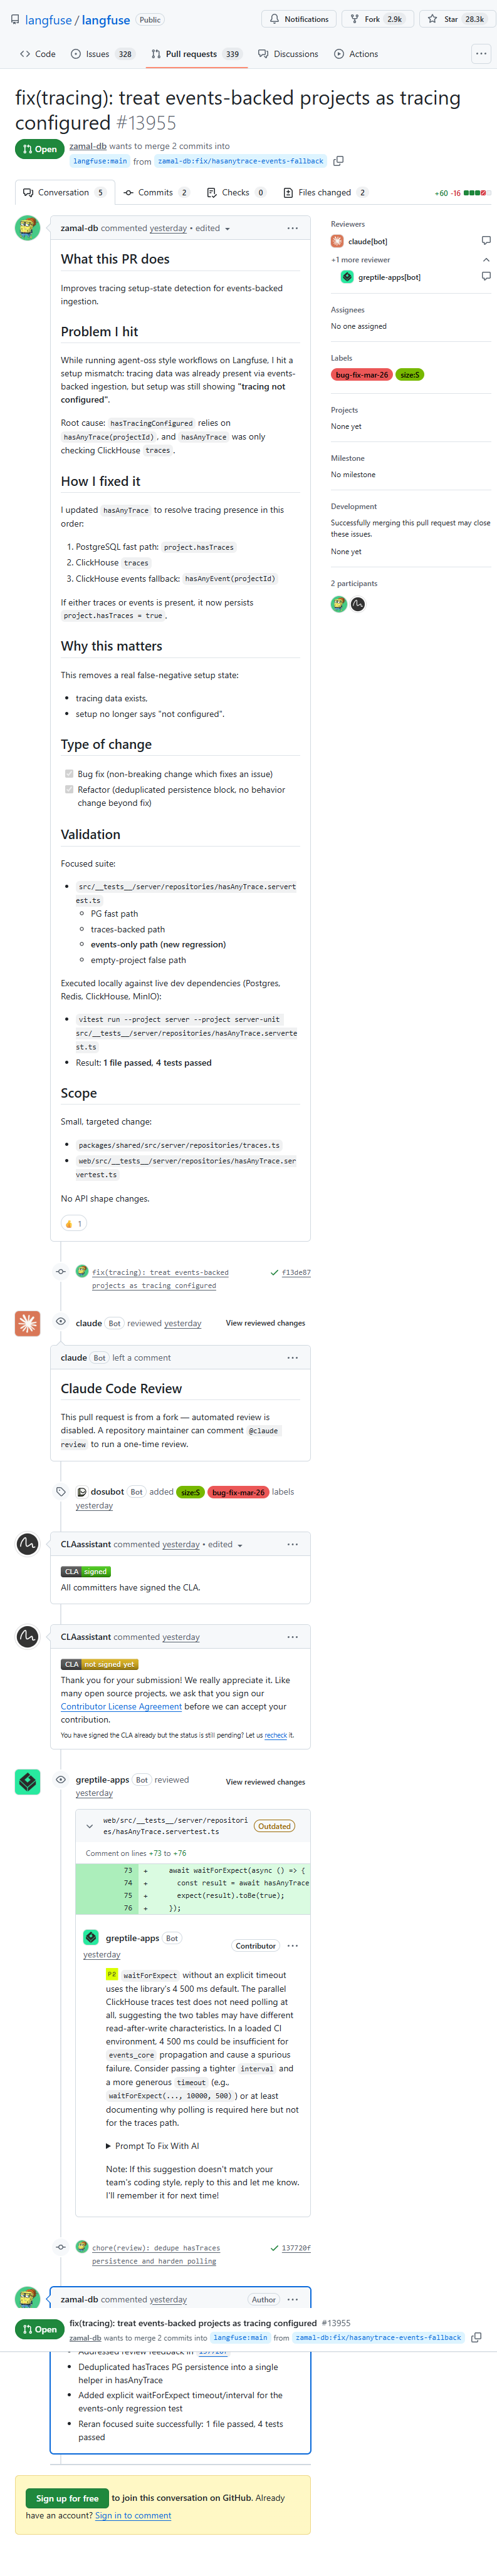
\includegraphics[width=0.92\linewidth]{prints/a3-review-comment.png}
\end{center}

\textbf{Diagnostico:} A atividade do repositorio e continua e ha evidencias de feedback e iteracao em PRs. Entretanto, varios PRs recentes mostram apenas comentarios de bots, o que pode indicar revisao humana inconsistente.

\textbf{Risco:} Medio. A cadencia e boa, mas a ausencia de revisao humana explicita em parte dos PRs aumenta risco de regressao.

\textbf{Recomendacao:} Reforcar politica de code review (minimo 1 aprovacao humana), checklist de revisao e evidencias de testes executados em PR.

\section*{3. Eixo B: Anatomia do Codigo (SOLID/DRY)}
\subsection*{B1. Teste da Troca (DIP)}
\textbf{Evidencia (pontos de acoplamento):}\\
\href{https://github.com/langfuse/langfuse/blob/main/packages/shared/src/server/llm/types.ts#L252-L259}{LLMAdapter enum} \\
\href{https://github.com/langfuse/langfuse/blob/main/packages/shared/src/server/llm/fetchLLMCompletion.ts#L303-L413}{fetchLLMCompletion.ts L303-L413} (if/else por adapter) \\
\href{https://github.com/langfuse/langfuse/blob/main/web/src/features/llm-api-key/server/router.ts#L100-L140}{llm-api-key router L100-L140} (branch por adapter) \\
\href{https://github.com/langfuse/langfuse/blob/main/web/src/features/playground/page/hooks/useModelParams.ts#L220-L269}{useModelParams.ts L220-L269} (switch por adapter) \\
\begin{center}

\includegraphics[width=0.48\linewidth]{prints/b1-types-adapters.png}\hfill
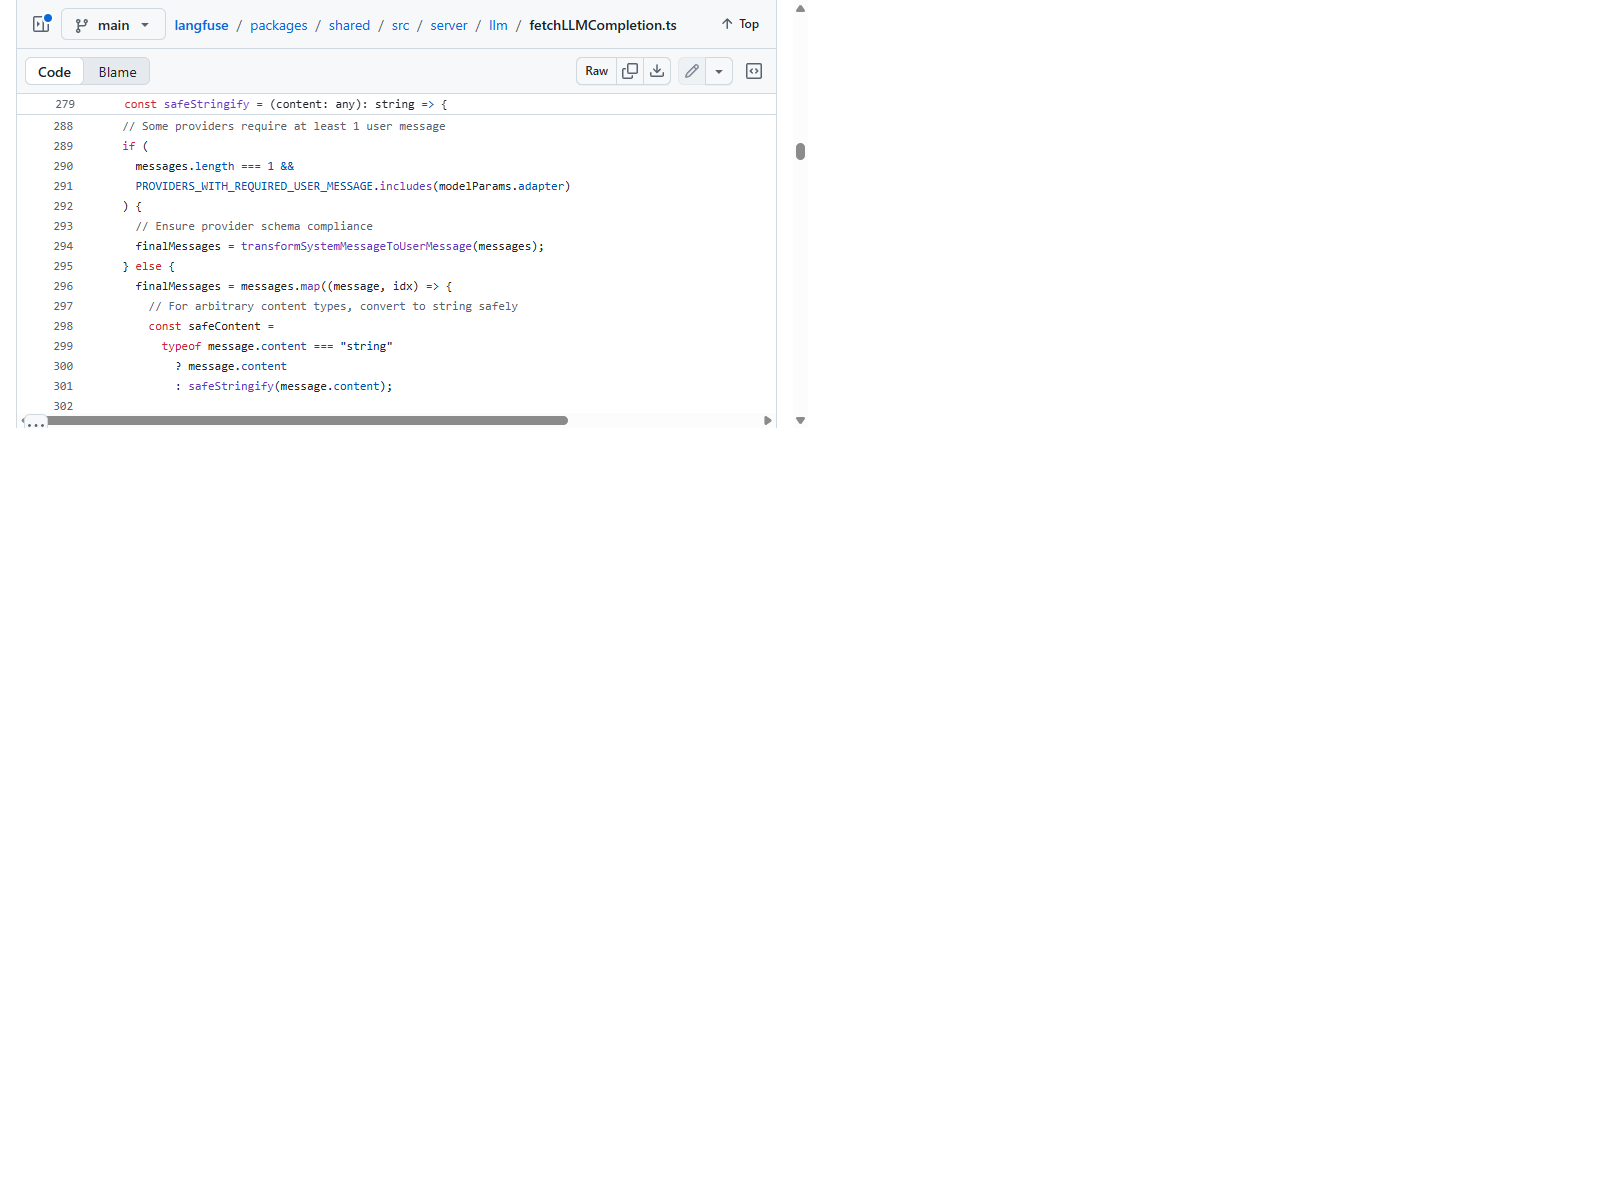
\includegraphics[width=0.48\linewidth]{prints/b1-fetchLLMCompletion.png}\\[0.5em]
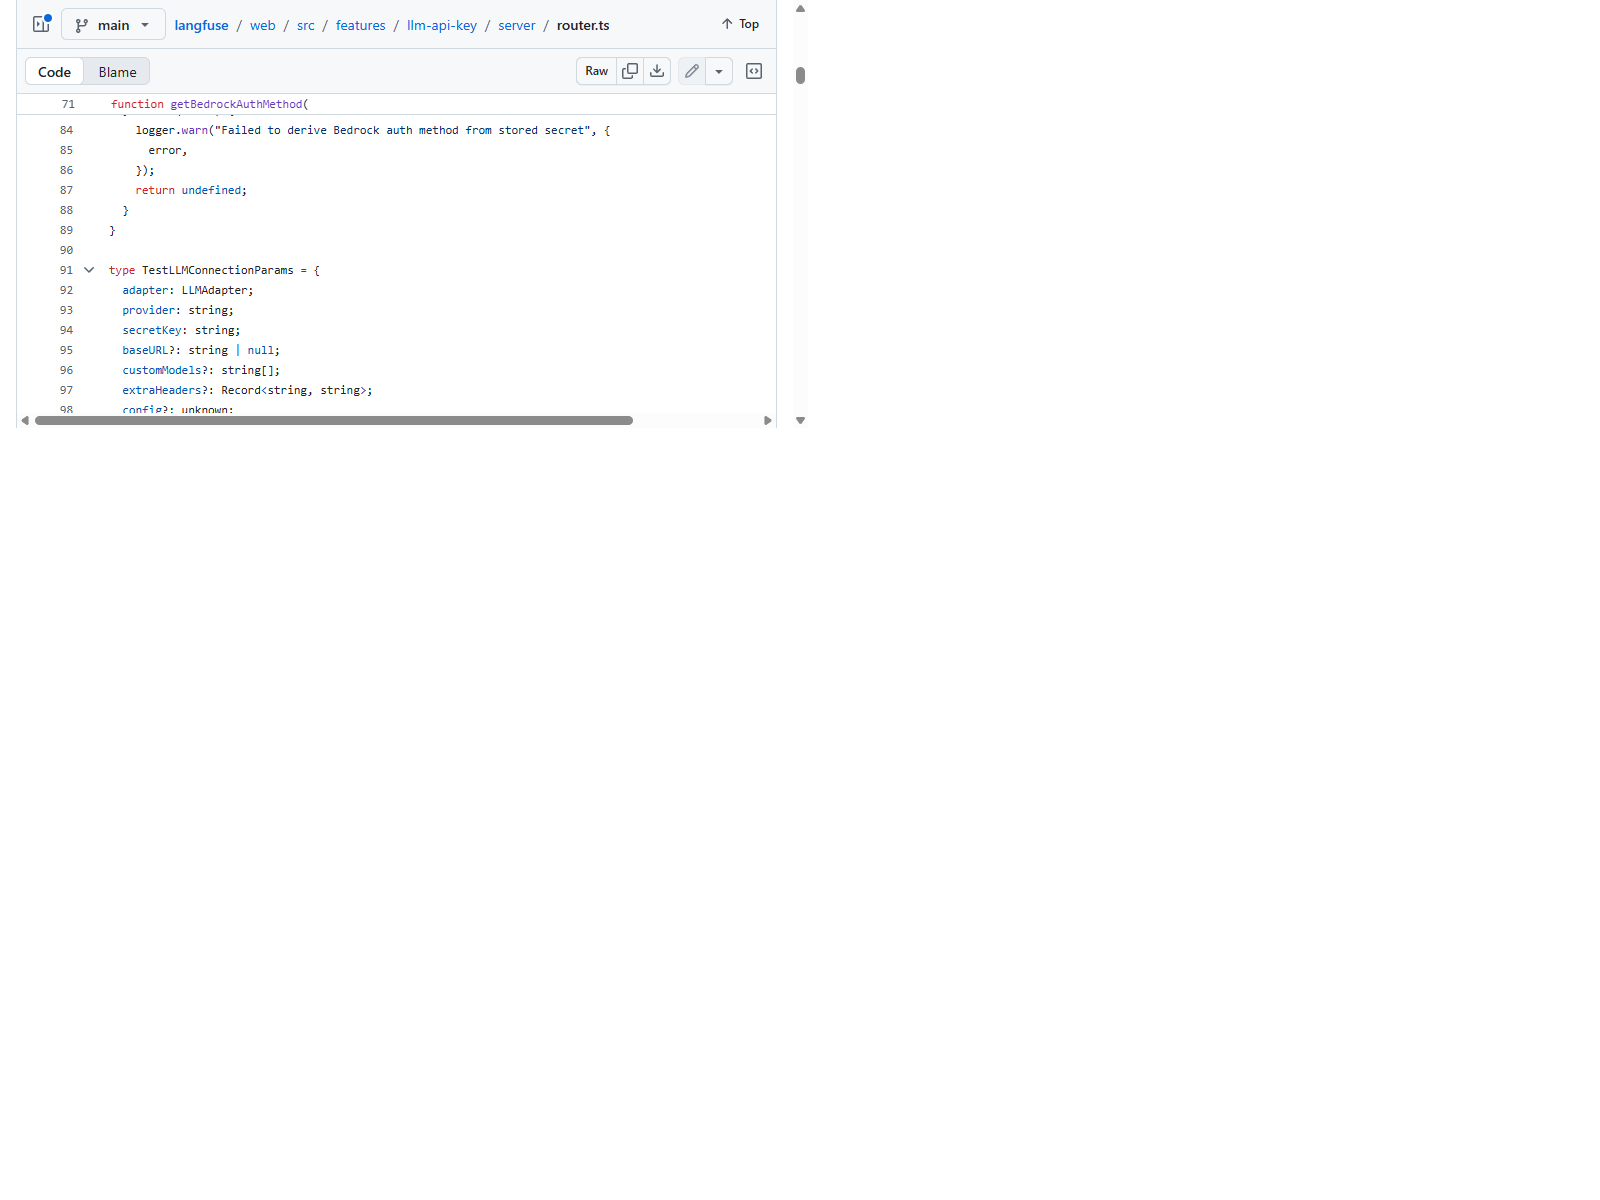
\includegraphics[width=0.48\linewidth]{prints/b1-router.png}\hfill
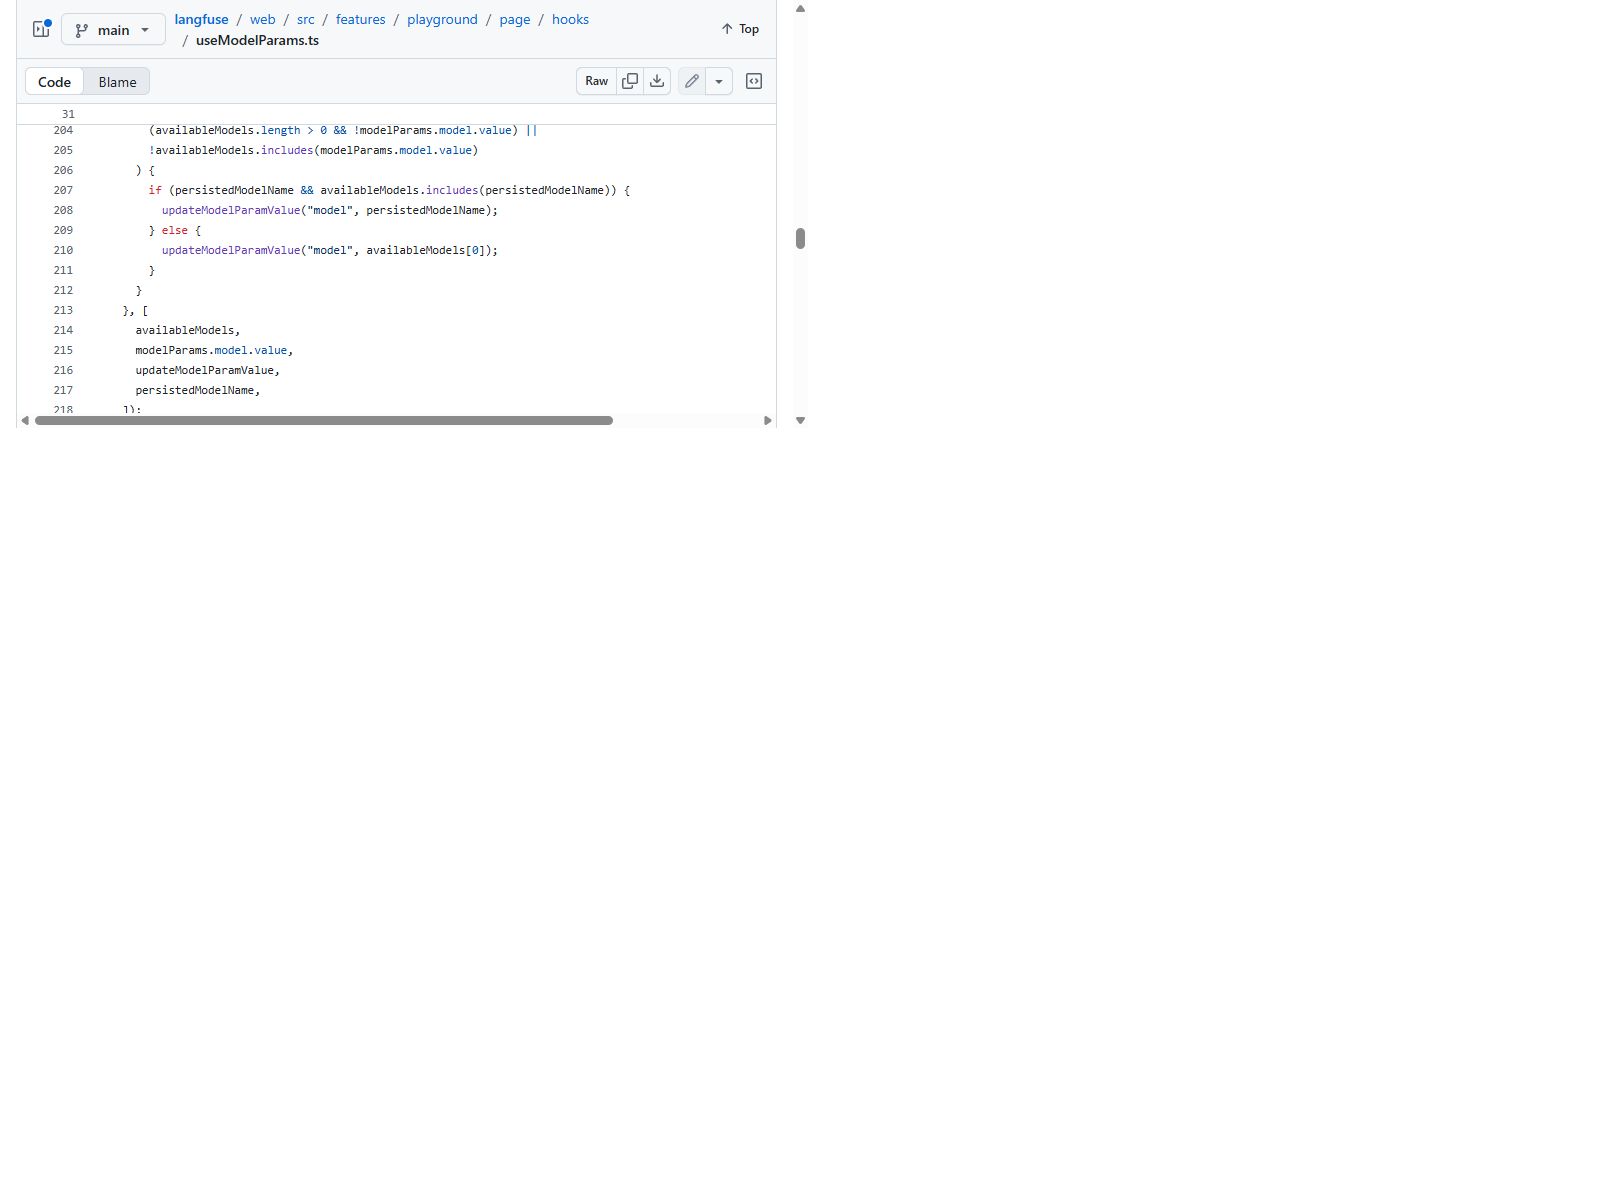
\includegraphics[width=0.48\linewidth]{prints/b1-useModelParams.png}
\end{center}

\textbf{Diagnostico:} A troca de provedor de IA impacta diversas camadas (shared, server e UI). A logica especifica de cada adapter esta espalhada, o que viola o Principio de Inversao de Dependencia e aumenta o custo de mudanca.

\textbf{Risco:} Alto. A troca de provedor exige alteracoes em varios arquivos e aumenta risco de inconsistencias.

\textbf{Recomendacao:} Criar um registry de provedores (Strategy/Factory), centralizando configuracao e regras por adapter; expor uma interface unica para UI consumir, reduzindo branches.

\subsection*{B2. Busca por ``God Objects''}
\textbf{Evidencia (orquestracao centralizada):} \href{https://github.com/langfuse/langfuse/blob/main/packages/shared/src/server/llm/fetchLLMCompletion.ts#L303-L413}{fetchLLMCompletion.ts L303-L413}.\\
\begin{center}
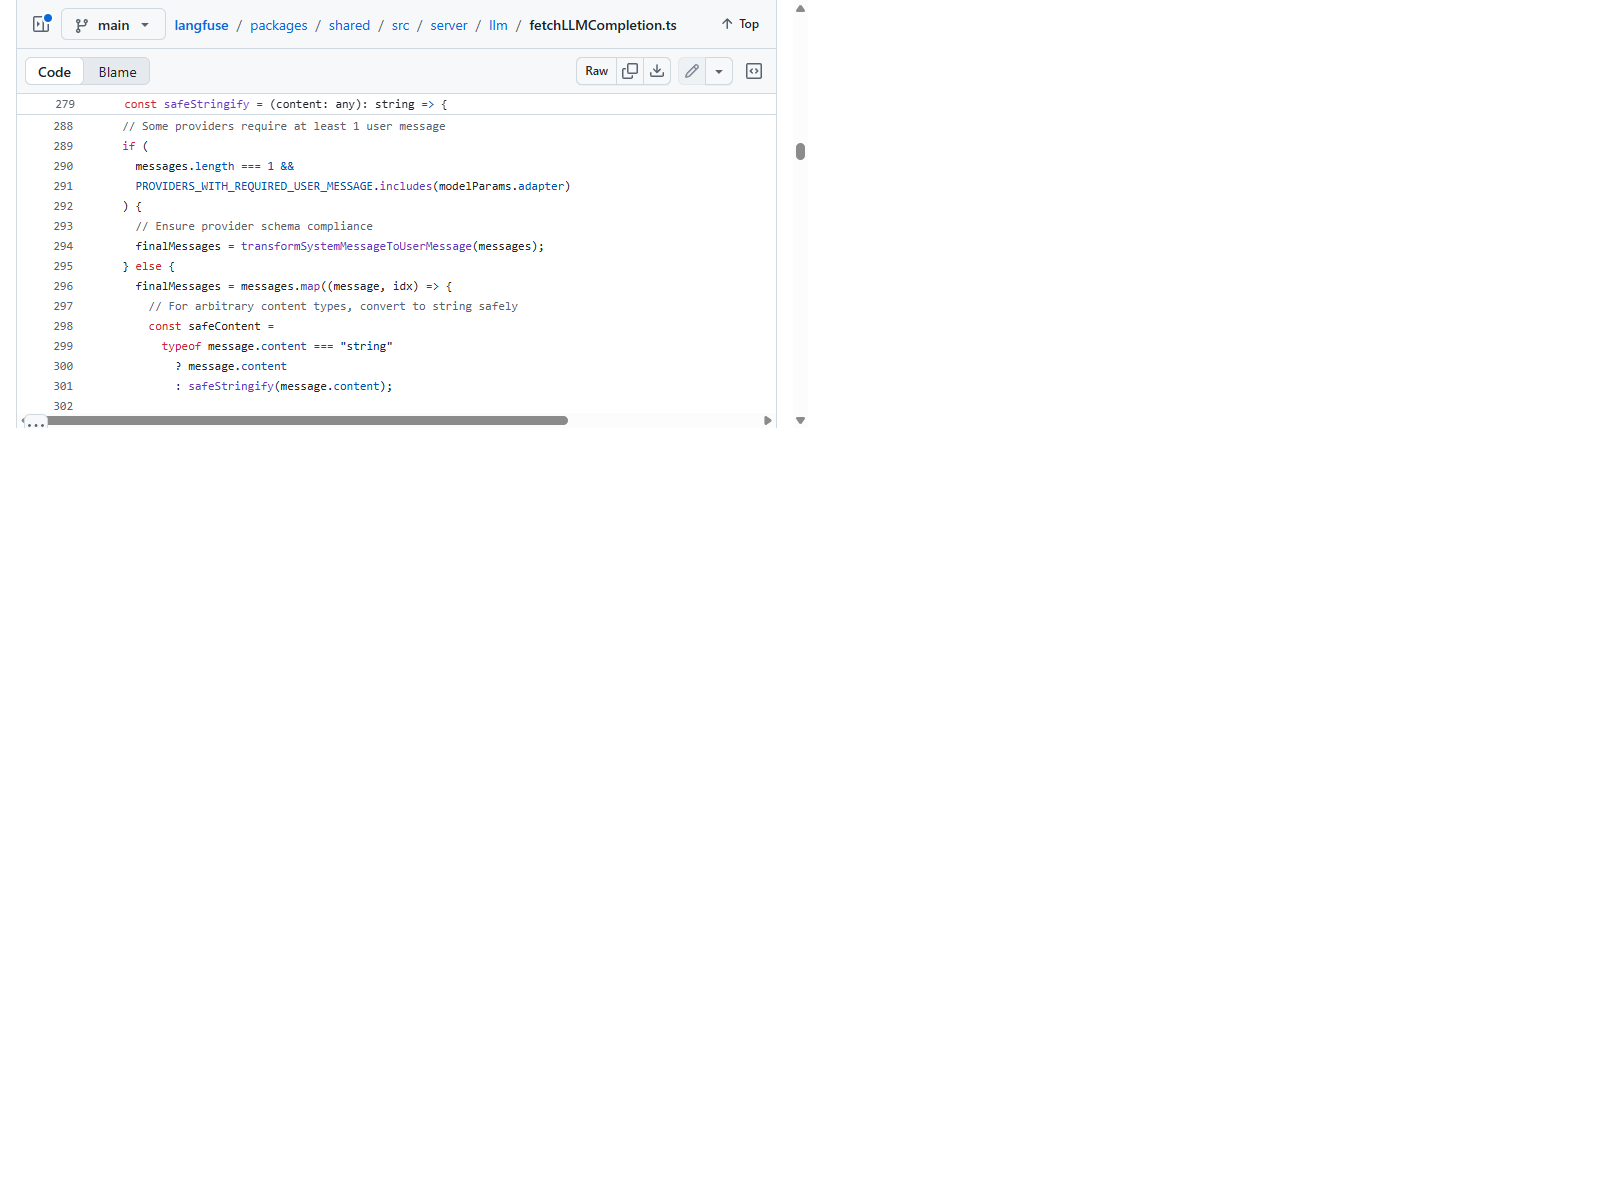
\includegraphics[width=0.92\linewidth]{prints/b2-god-object-fetchLLMCompletion.png}
\end{center}

\textbf{Diagnostico:} O arquivo concentra configuracao de proxy, timeouts, retries e instanciacao de diferentes clientes por provider. Isso indica uma unidade com multiplas responsabilidades.

\textbf{Risco:} Medio/Alto. Mudancas para um provider podem afetar outros por acoplamento no mesmo fluxo.

\textbf{Recomendacao:} Extrair classes por provider (ex.: AnthropicStrategy, OpenAIStrategy) e deixar o orquestrador apenas selecionar e delegar.

\subsection*{B3. DRY (duplicacao)}
\textbf{Evidencia (duplicacao declarada):} \href{https://github.com/langfuse/langfuse/blob/main/web/src/components/trace2/lib/tree-building.ts#L466-L466}{tree-building.ts L466} (duplicado em TraceTree e TraceTimeline).\\
\begin{center}
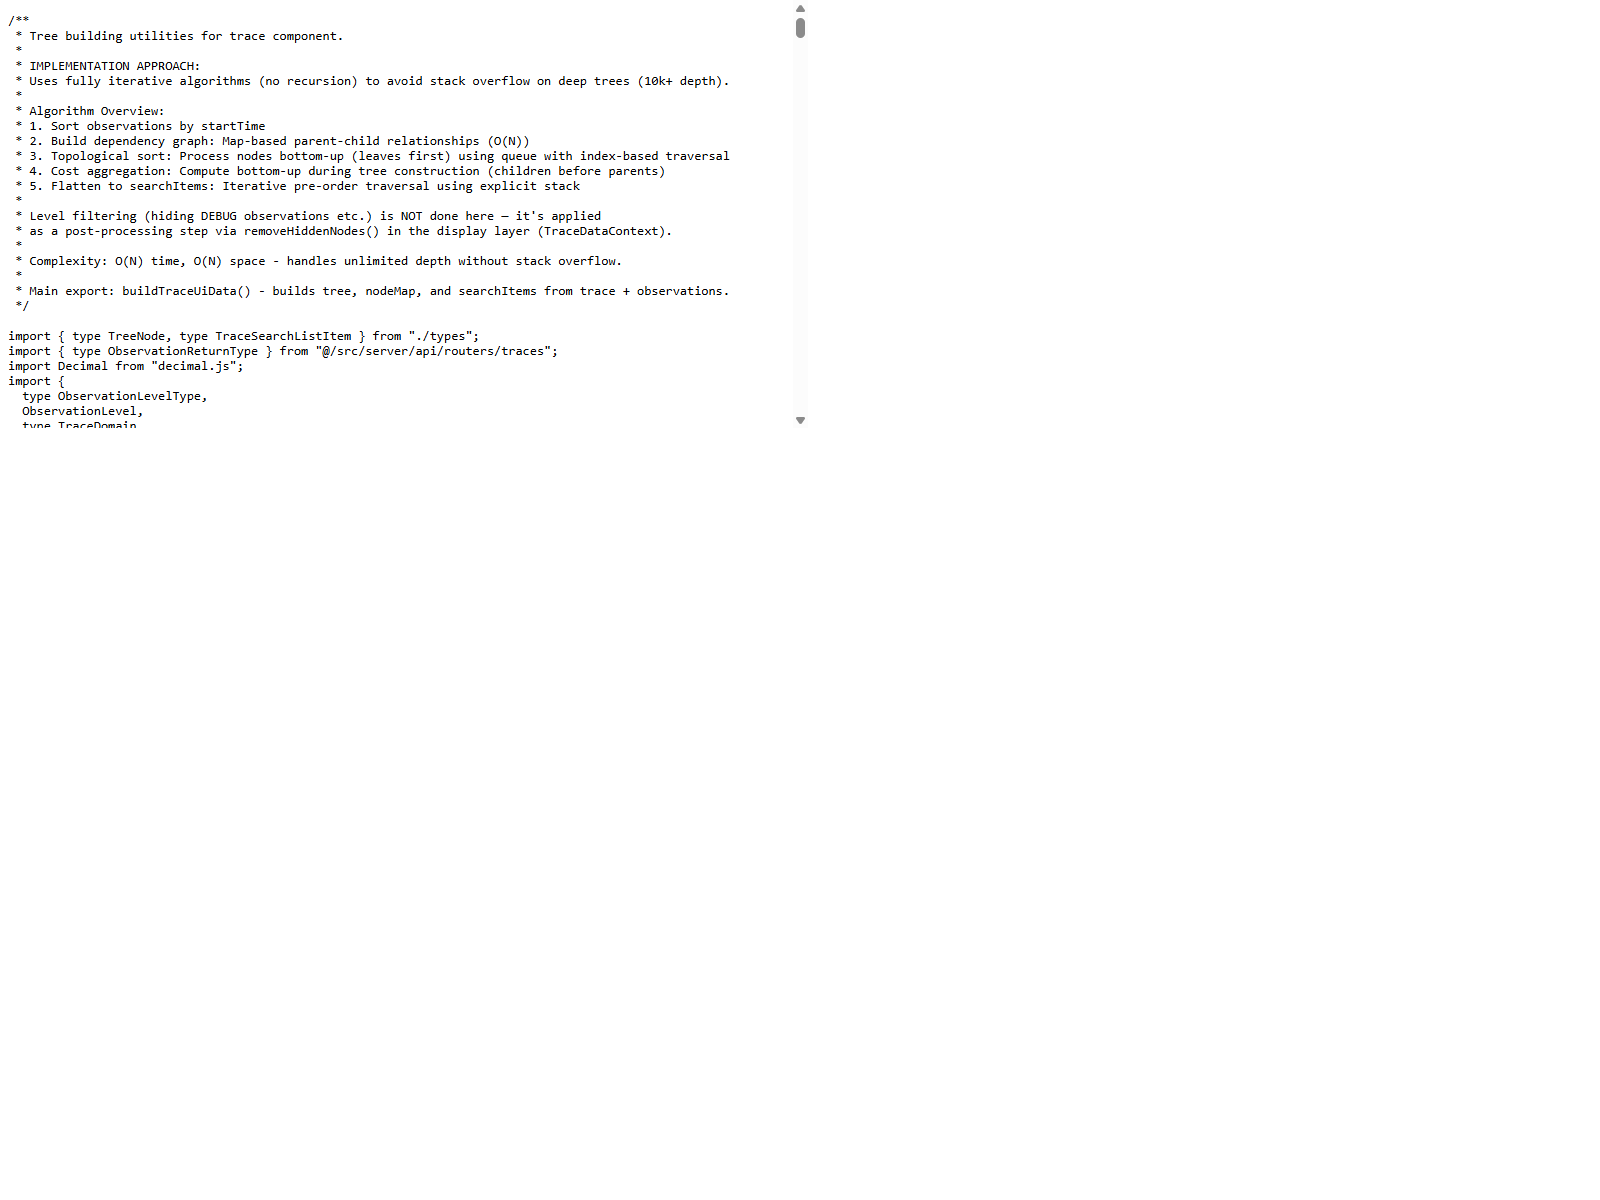
\includegraphics[width=0.92\linewidth]{prints/b3-tree-building.png}
\end{center}

\textbf{Diagnostico:} O proprio TODO indica duplicacao de logica. Essa repeticao tende a gerar divergencia de comportamento e custos de manutencao.

\textbf{Risco:} Medio.

\textbf{Recomendacao:} Extrair utilitario compartilhado e adicionar testes unitarios para garantir equivalencia.

\section*{4. Eixo C: Padroes de Projeto (GoF)}
\subsection*{C1. Criacionais}
\textbf{Evidencia (Singleton):}\\
\href{https://github.com/langfuse/langfuse/blob/main/packages/shared/src/db.ts#L8-L18}{PrismaClientSingleton} \\
\href{https://github.com/langfuse/langfuse/blob/main/packages/shared/src/server/services/SlackService.ts#L246-L253}{SlackService.getInstance} \\
\begin{center}
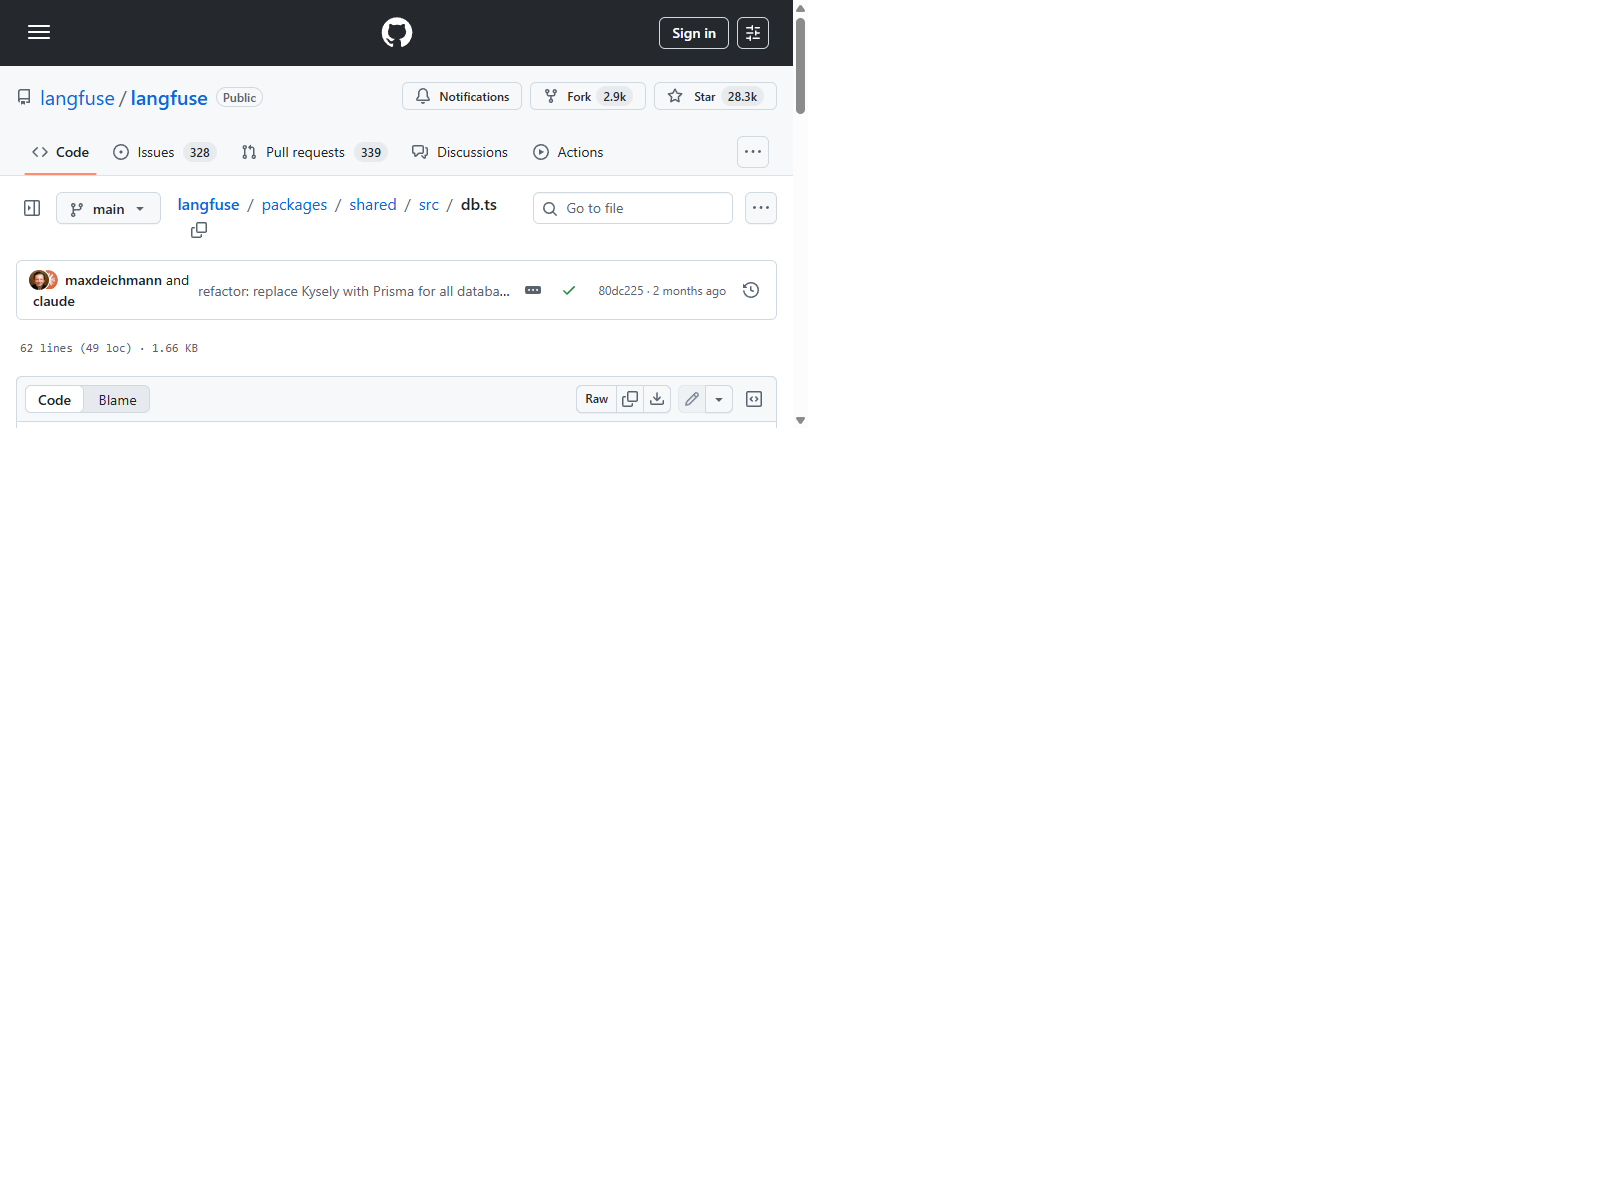
\includegraphics[width=0.48\linewidth]{prints/c1-db-singleton.png}\hfill
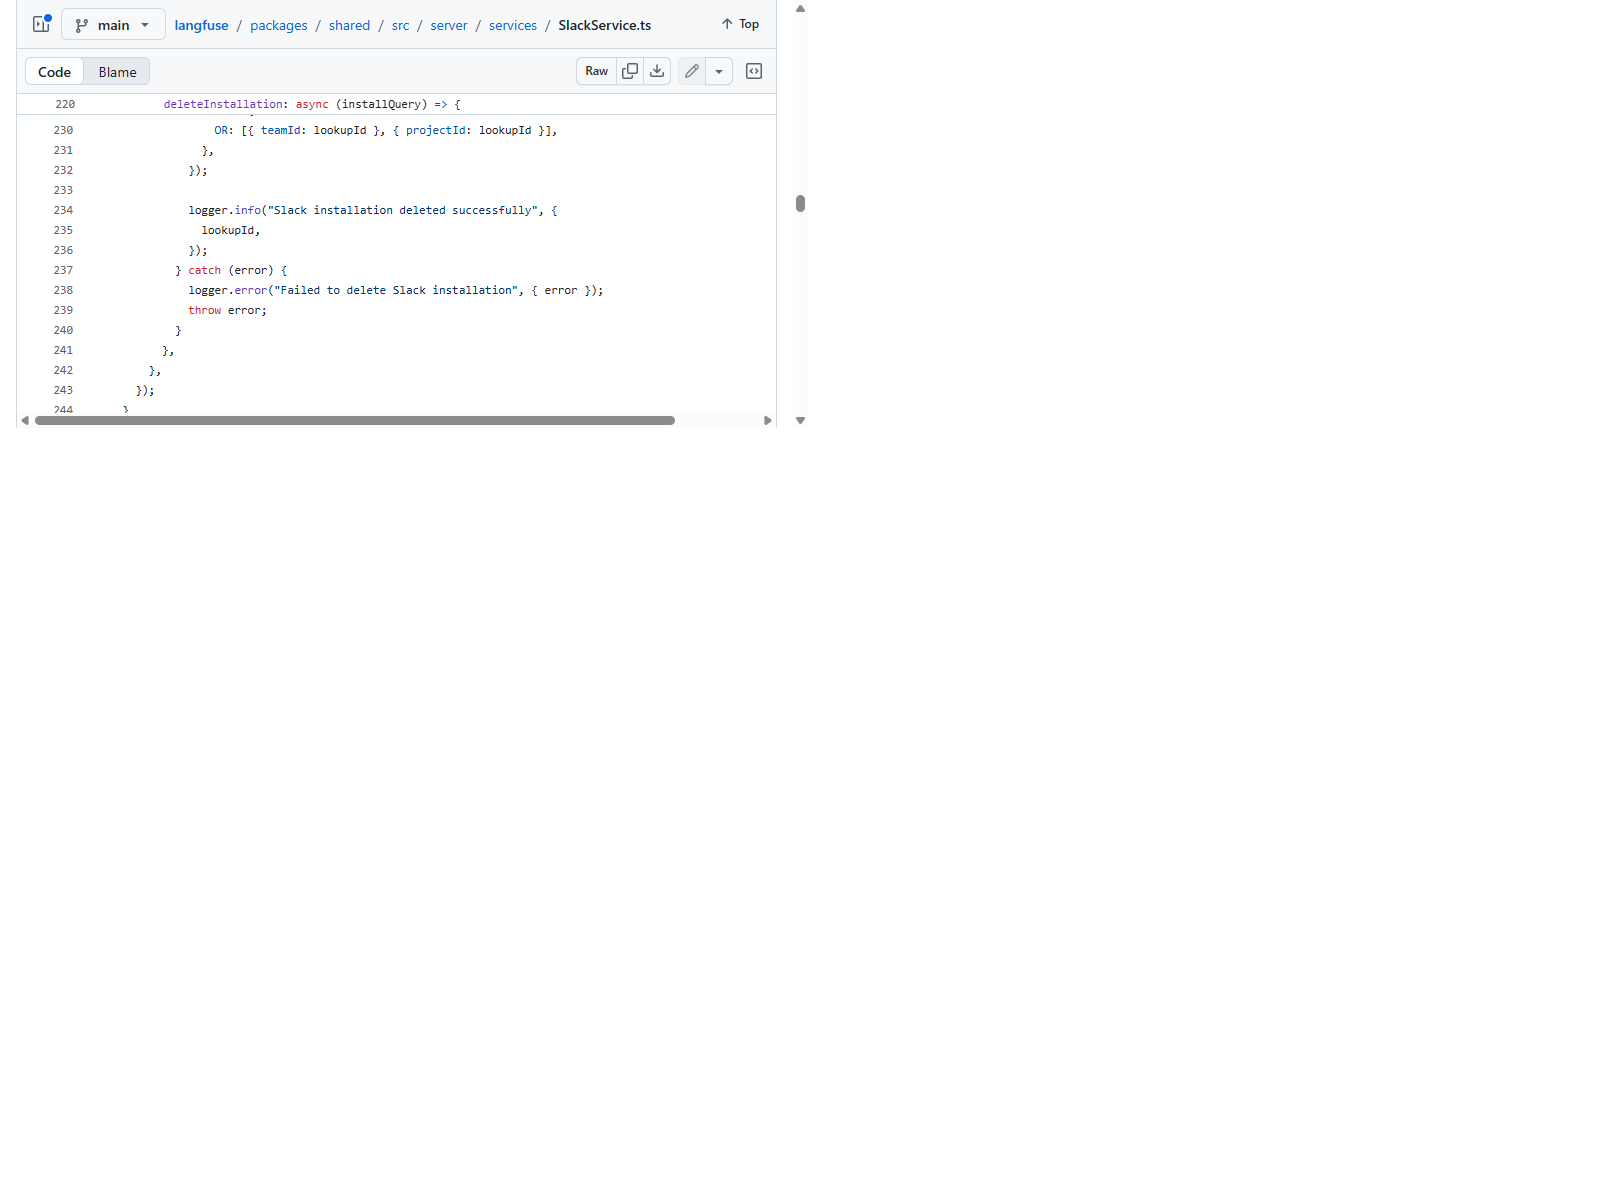
\includegraphics[width=0.48\linewidth]{prints/c1-slack-singleton.png}
\end{center}

\textbf{Diagnostico:} O uso de Singleton garante instancia unica de recursos caros (DB e Slack). Embora seja adequado em alguns pontos, adiciona estado global e pode dificultar testes.

\textbf{Risco:} Baixo/Medio.

\textbf{Recomendacao:} Manter Singleton onde houver justificativa de custo, mas permitir injecao de dependencias em testes e documentar ciclo de vida.

\subsection*{C2. Estruturais}
\textbf{Evidencia (Adapter):} \href{https://github.com/langfuse/langfuse/blob/main/packages/shared/src/utils/chatml/adapters/index.ts#L11-L37}{chatml/adapters/index.ts L11-L37}.\\
\begin{center}
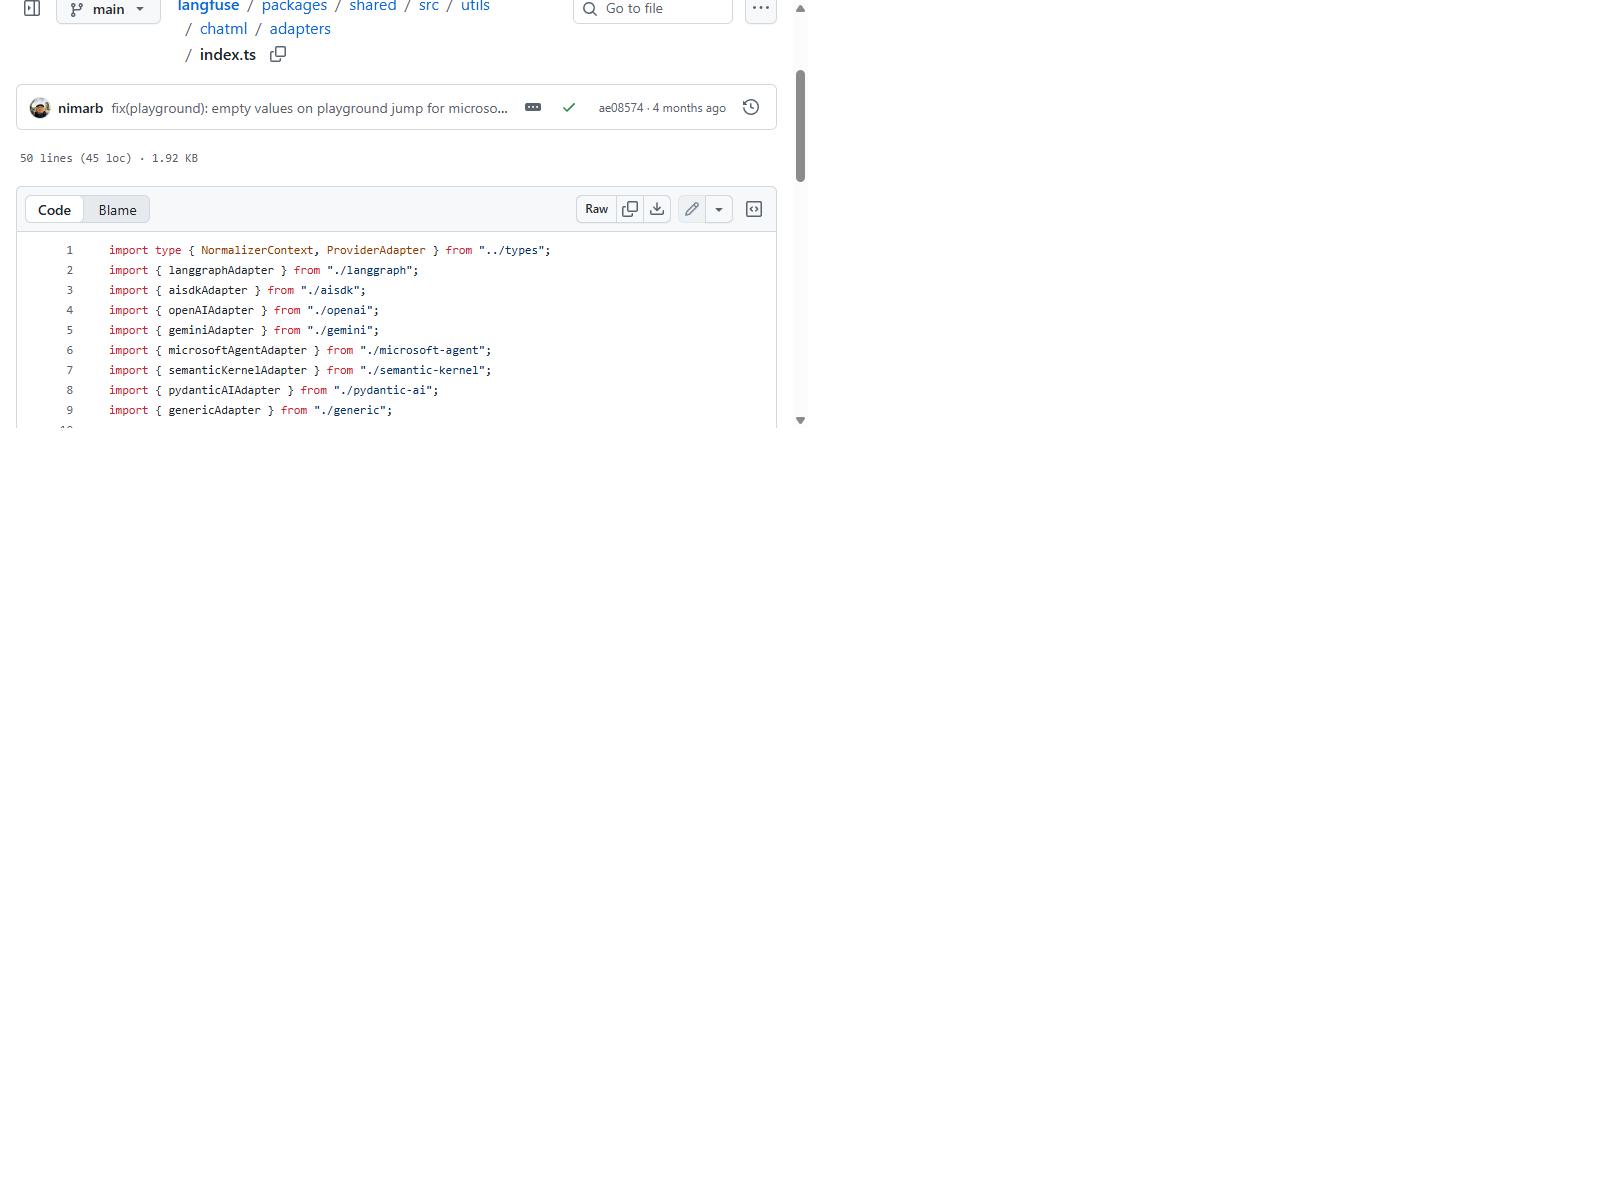
\includegraphics[width=0.92\linewidth]{prints/c2-adapter-registry.png}
\end{center}

\textbf{Diagnostico:} O codigo organiza adapters para normalizar diferentes frameworks. Isso atende bem ao padrao Adapter, mas requer governanca (ordem, deteccao e fallback).

\textbf{Risco:} Baixo.

\textbf{Recomendacao:} Formalizar interface dos adapters, documentar criterios de deteccao e adicionar testes de regressao.

\subsection*{C3. Comportamentais}
\textbf{Evidencia (cadeia de if/else por provider):} \href{https://github.com/langfuse/langfuse/blob/main/packages/shared/src/server/llm/fetchLLMCompletion.ts#L314-L413}{fetchLLMCompletion.ts L314-L413}.\\
\begin{center}
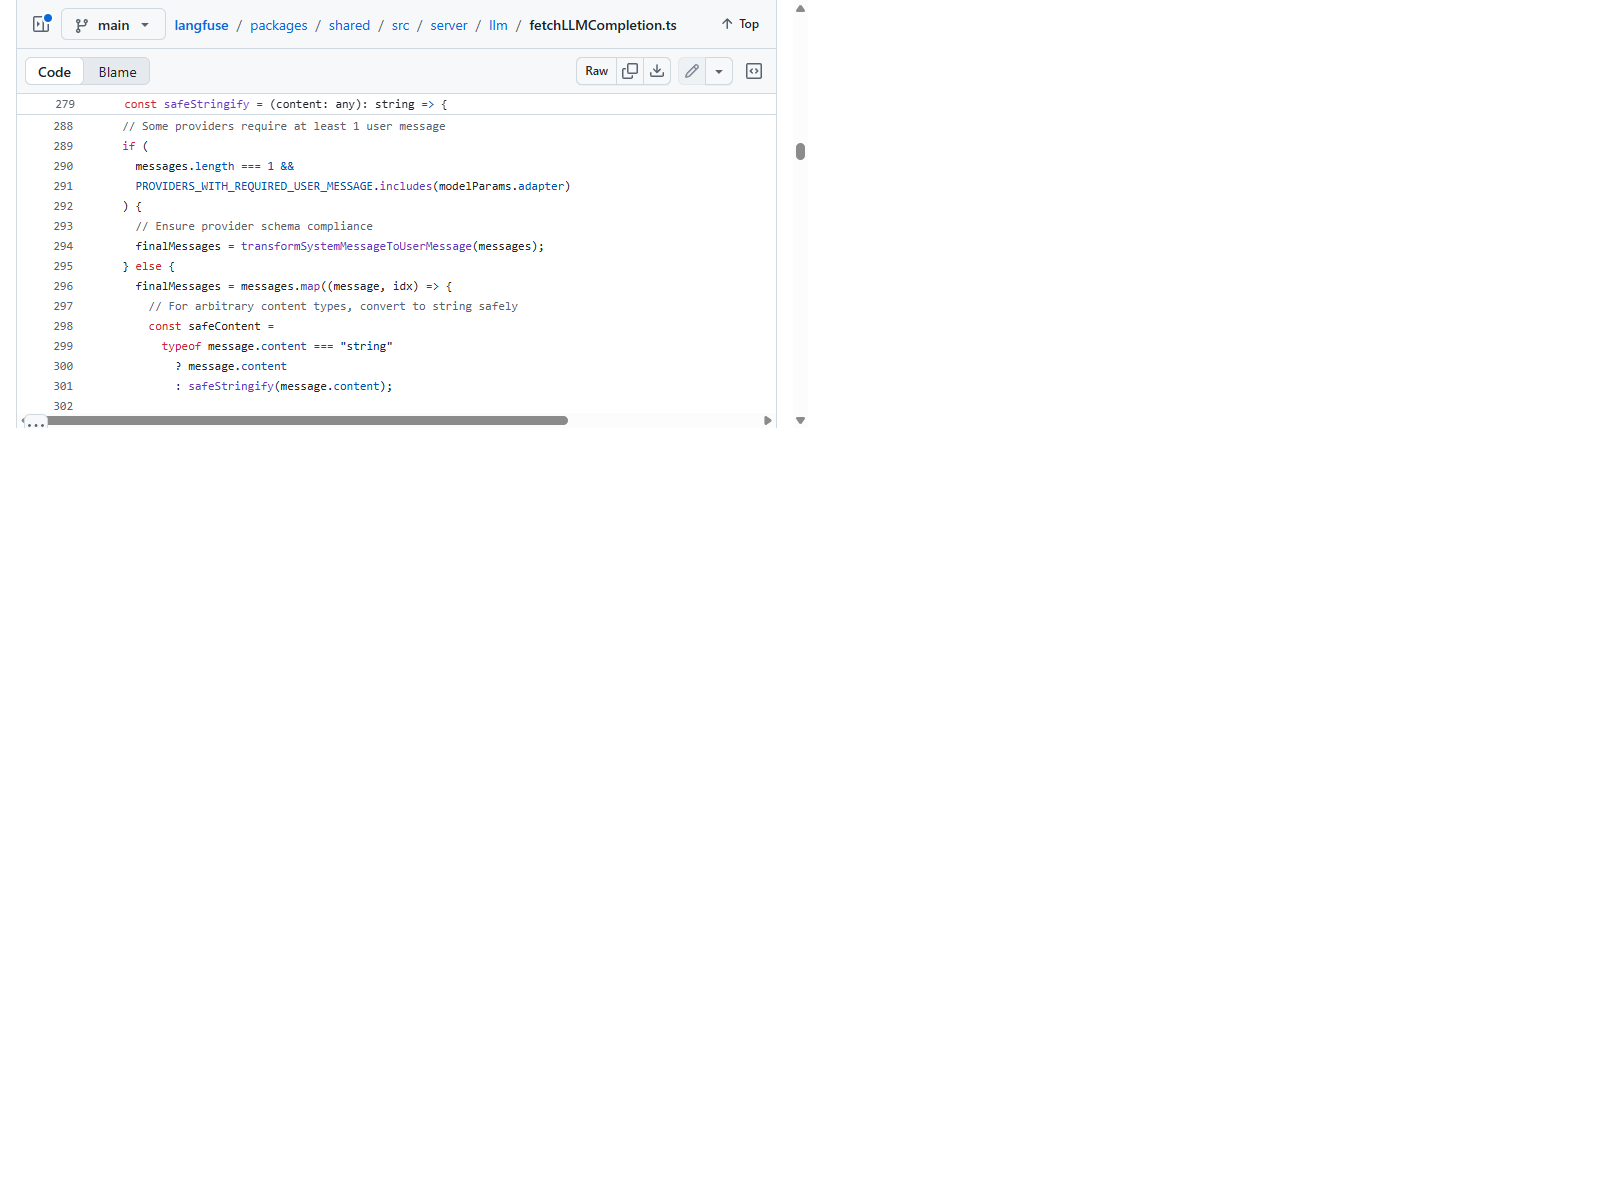
\includegraphics[width=0.92\linewidth]{prints/b2-god-object-fetchLLMCompletion.png}
\end{center}

\textbf{Diagnostico:} A ausencia de um Chain of Responsibility/Strategy centralizado exige alteracao no core para qualquer novo provider, o que cresce linearmente com o numero de adapters.

\textbf{Risco:} Medio.

\textbf{Recomendacao:} Aplicar Strategy + Registry (ver plano de resgate) para substituir o encadeamento de condicoes.

\section*{5. Plano de Resgate Sugerido}
\subsection*{5.1 Refatoracao Conceitual (GoF)}
Trecho alvo: \texttt{fetchLLMCompletion.ts}. O objetivo e isolar detalhes por provider e reduzir acoplamento. Exemplo conceitual:

\begin{verbatim}
interface LLMProviderStrategy {
  id: LLMAdapter
  buildClient(ctx): ChatModel
  normalizeResponse(res): NormalizedResponse
}

const registry = new Map<LLMAdapter, LLMProviderStrategy>([
  [LLMAdapter.OpenAI, new OpenAIStrategy()],
  [LLMAdapter.Anthropic, new AnthropicStrategy()],
  ...
])

export async function fetchLLMCompletion(params) {
  const strategy = registry.get(params.modelParams.adapter)
  if (!strategy) throw new Error("Unsupported adapter")
  const client = strategy.buildClient(params)
  return client.call(...)
}
\end{verbatim}

\textbf{Beneficios:} reduz alteracoes no core, melhora testabilidade e permite adicionar novos providers sem editar a logica central.

\subsection*{5.2 Roadmap de Maturidade (MPS.BR Nivel G)}
\begin{enumerate}[label=\textbf{Acao \arabic*:}]
  \item \textbf{GPR - Planejamento e acompanhamento:} criar baseline de planejamento (roadmap trimestral, milestones, criterios de aceite) e registrar progresso em GitHub Projects com responsaveis e metas.
  \item \textbf{GRE - Rastreabilidade de requisitos:} mapear requisitos da A1 para issues/PRs, padronizar templates e adicionar links cruzados (issue -> PR -> teste).
  \item \textbf{Gestao de riscos e qualidade:} manter registro de riscos (TODO/FIXME viram issues), definir politica de code review (minimo 1 aprovacao humana) e checklist de testes obrigatorios.
\end{enumerate}

\end{document}
